\section{TORCS (The Open Racing Car Simulator)}
\label{sec:TORCS}
The environment to use in reinforcement learning is important, because it is here all the learning will be done. This project is using reinforcement learning in autonomous driving. After reading the post \cite{DDPG_Torcs} that uses TORCS in combination with Gym-TORCS. It was decided that this project will use the same environment, because it seems like it will make a good simulation environment for the task in the project. It is also an environment DeepMind has used to test their algorithms \cite{DBLP:journals/corr/LillicrapHPHETS15} and \cite{DBLP:journals/corr/MnihBMGLHSK16}, it is thereby a well-known environment to use in reinforcement learning. 

The Open Racing Car Simulator or TORCS is a highly portable multi-platform car racing simulation. It is used as ordinary car racing game, as AI racing game and as a research platform. The source code of TORCS is licensed under the GPL ("Open Source") \cite{TORCS_website}. 

Gym-TORCS is a reinforcement learning environment in the TORCS domain. It is made to have an interface which matched Open-AI - A toolkit for developing and comparing reinforcement learning algorithms. It supports teaching agents everything from walking to playing games like Pong or Go \cite{OPENAI_website}. It is smart to match the Open-AI interface because it combines a lot of environment to solve different reinforcement learning tasks. This is done by a simple interface to make it easier to use. \cite{Gym_TORCS_website}. 

Some points why TORCS is useful as an environment for reinforcement learning:
\begin{itemize}
	\item The AI can learn how to drive
	\item It is possible to visualize how the neural networks learn over time and inspect its learning process. Instead of only looking at the final result.
	\item It is easy to visualize when the neural network gets stuck in a local minimum.
	\item Gives an understanding of machine learning technique in automated driving, which is important for autonomous driving technologies 
\end{itemize}

Some pictures from TORCS can be found on \Cref{fig:torcs_screenshots} the below:
\begin{figure} [H]
	\centering
	\begin{subfigure}{.20\textwidth}
		\centering
		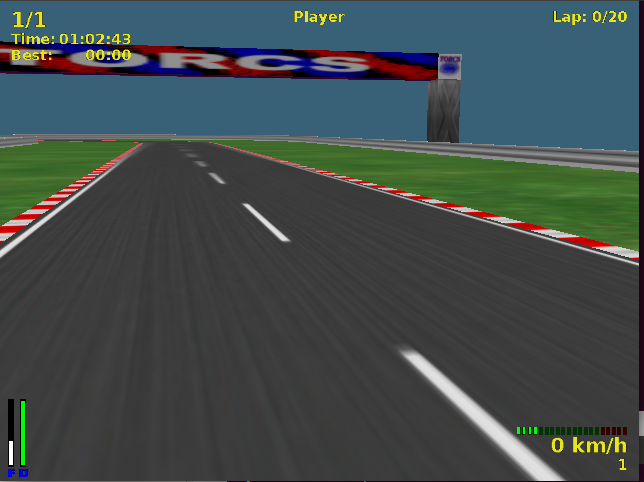
\includegraphics[width=25mm, height=25mm]{Figures/Architecture/Torcs/torcs_2.png}
	\end{subfigure}
	\begin{subfigure}{.20\textwidth}
	\centering
	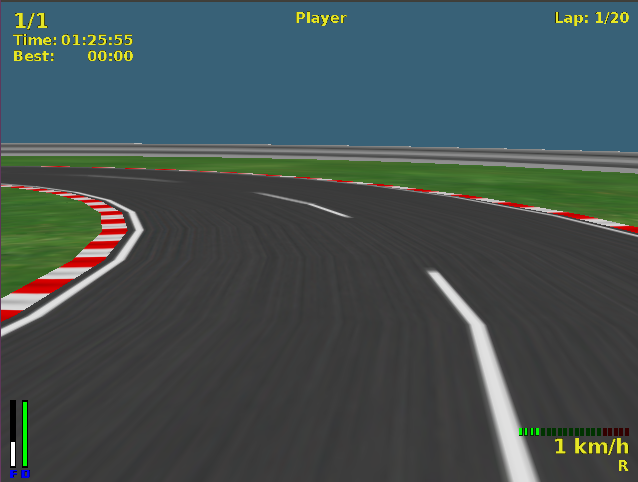
\includegraphics[width=25mm, height=25mm]{Figures/Architecture/Torcs/torcs_3.png}
    \end{subfigure}
	\begin{subfigure}{.20\textwidth}
	\centering
	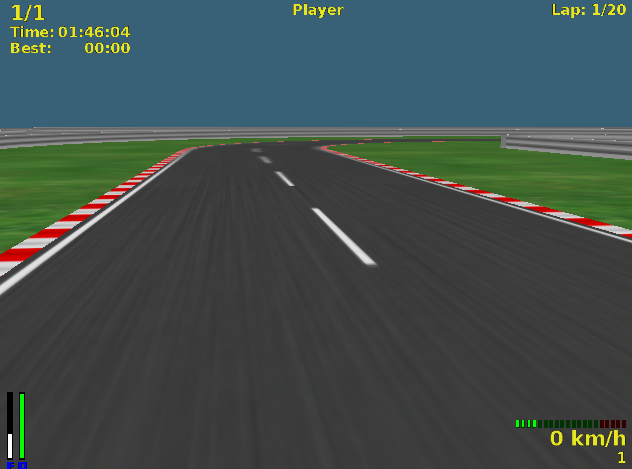
\includegraphics[width=25mm, height=25mm]{Figures/Architecture/Torcs/torcs_4.png}
	\end{subfigure}
	\begin{subfigure}{.20\textwidth}
	\centering
	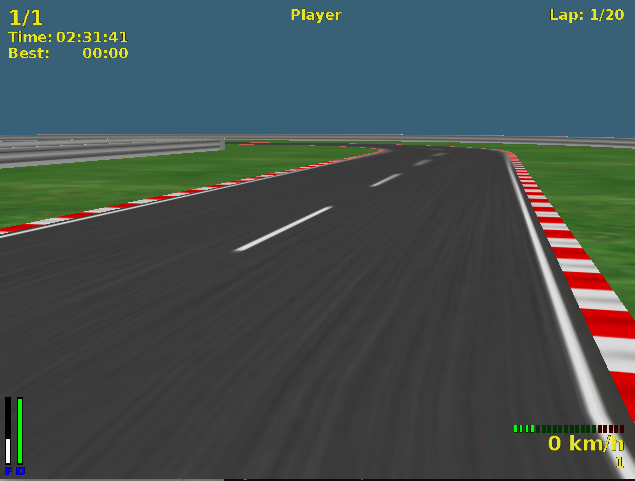
\includegraphics[width=25mm, height=25mm]{Figures/Architecture/Torcs/torcs_5.png}
	\end{subfigure}
	\caption{Screenshots from the TORCS environment}
	\label{fig:torcs_screenshots}
\end{figure}
      
\subsection{Uses in this project}      
The way this environment has been used, is by getting information from the TORCS domain. This information could be the game screen, so the pixels of the game. Another thing the environment has been used for, is to send commands to the game - like steering the car. 

The reinforcement learning should be able to train a network, where the input to the network is the information coming from the game. The output from the network is the determined action, which then will be send to the game. This interaction between the game and the network can be seen on \Cref{fig:TORCS_interaction}.    
 
\begin{figure}[H]
	\centering
	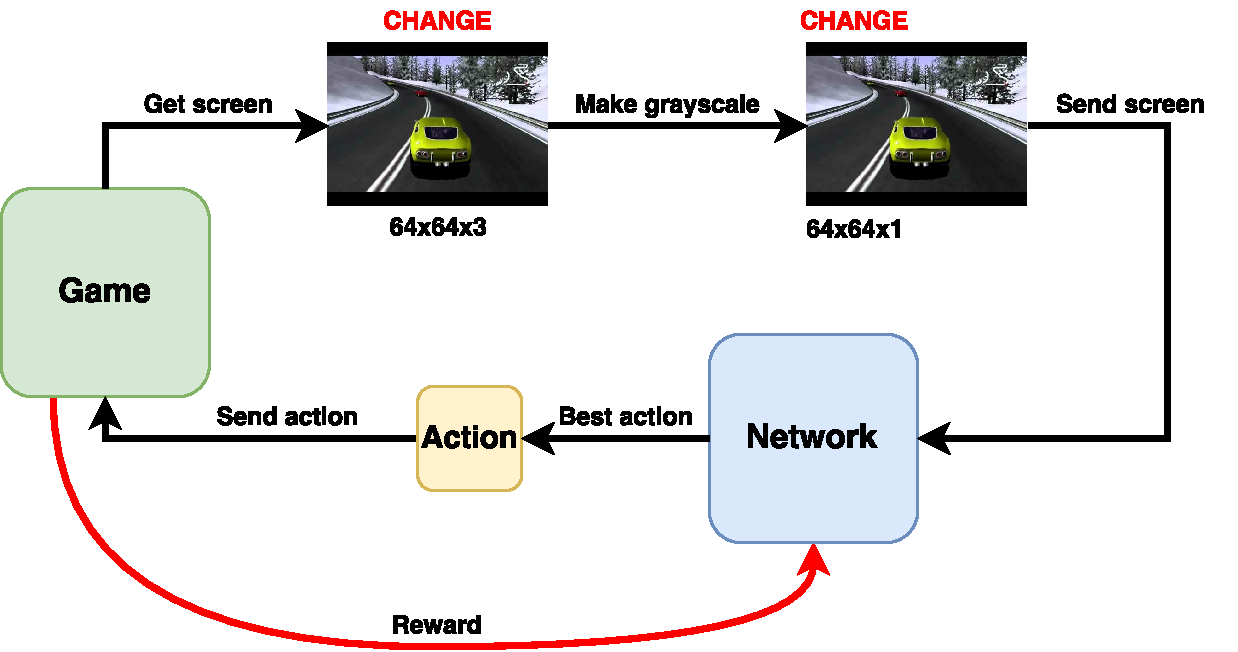
\includegraphics[width=1\textwidth]{Figures/Architecture/TORCS_interaction.pdf}
	\caption{The interaction between the game (TORCS) and the network }
	\label{fig:TORCS_interaction}
\end{figure}

 
As seen on \Cref{fig:TORCS_interaction} the screen is taken from the game, which in this project is TORCS. The screen is the state in our reinforcement learning algorithm. The image screen in this case is of size $64 \times 64$ and have three color channels - red, green and blue. Then some preprocessing is happening for getting this image to the right format, so the network can analyze it. 

 The preprocessing of the image, is to make the image to grayscale. This is done by taken the RGB-image array ($64 \times 64 \times 3$) and separate the 3 color channels red, green and blue. These RGB-values is converted to grayscale values by forming a weighted sum of the R, G and B components:

\begin{equation}
grayscale = 0.2989 \cdot R + 0.5870 \cdot G + 0.1140 \cdot B 
\end{equation}  

The network will then take $64 \times 64 $ image as inputs, more about the network used in this project is described in \Cref{sec:A3C}. The network then uses this input to find the best action, in this state (screen of the game). 

The action the network has found, is then send to the game. The game will then behave after this action and send a reward back to the network. This reward is used to learn the network how to play the game - this is also called training of the network. This procedure continues until the maximum reward is achieved.   
 

 

 
   